\section{The Shallow Water Equations in Spherical Coordinates}
Until now we have derived the shallow water equations in cartesian coordinates.
In this section, we will derive the SWE in spherical coordinate, which is necessary if we want to model water flow on Earth.
We will follow the methods used in~\cite{Castro2017}~\cite{Bihlo2022},~\cite{Raymond} and~\cite{Gill_1982}.
To illustrate the spherical coordinates, we will use the latitude and longitude system, visualized in~\autoref{fig:lat-long-earth}.
\begin{figure}[H]
    \centering
    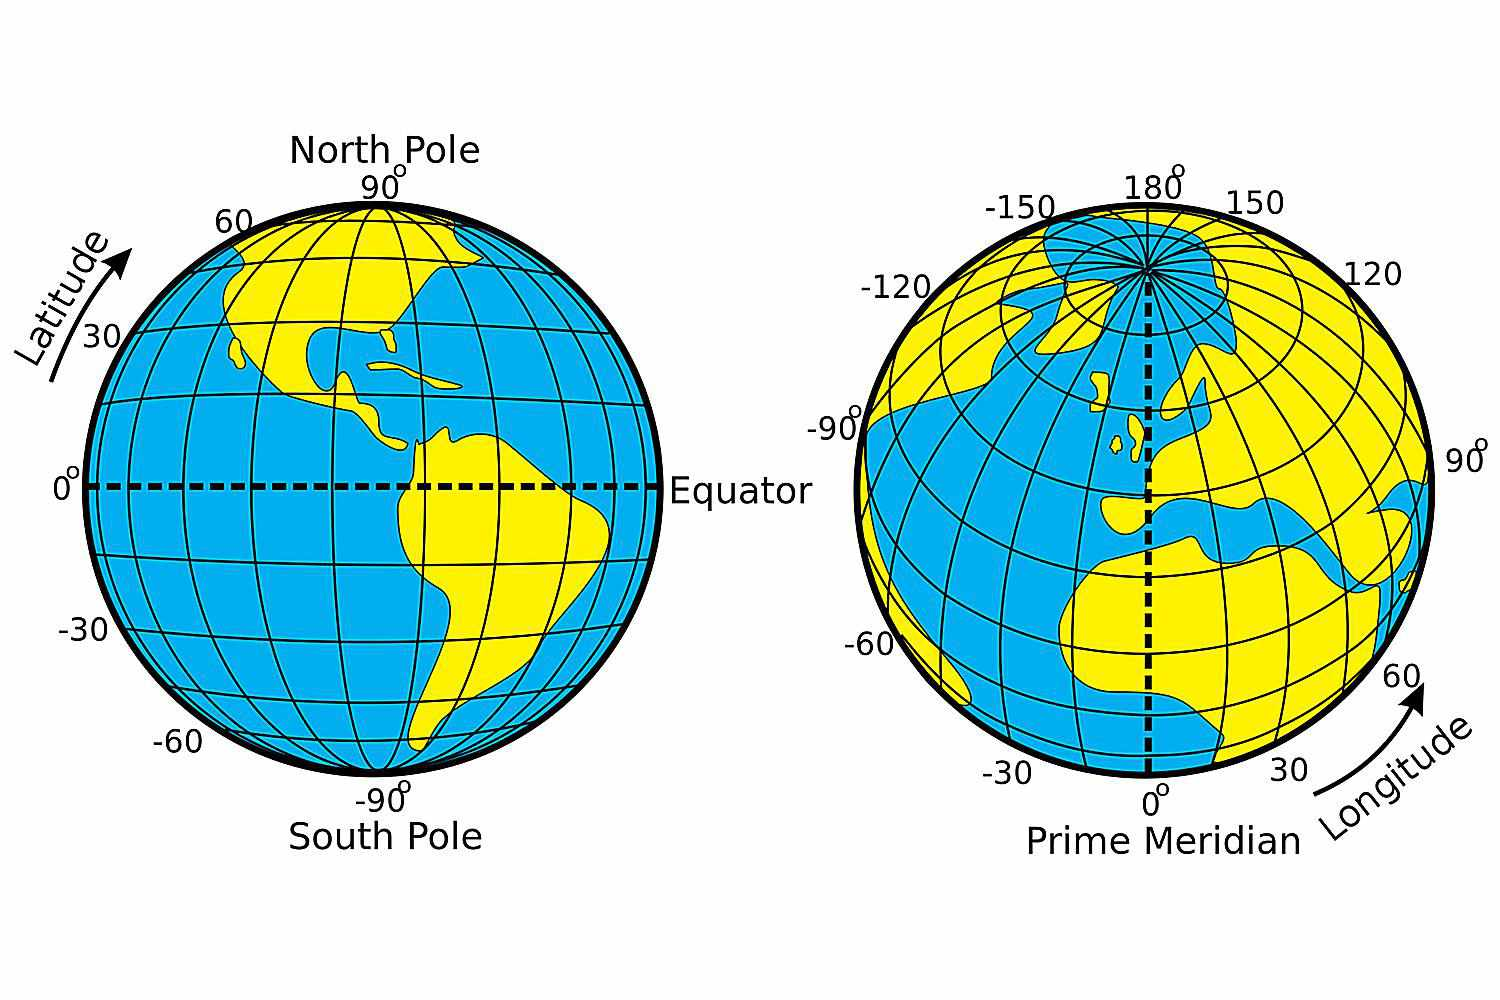
\includegraphics[width=0.5\textwidth]{C:/Users/Matteo/Shallow-Water-Equations/figs/lat-long-earth.jpg}
    \caption{Illustration of the latitude and longitude system for the planet earth.
    Illustration from~\cite{lat-long-earth}.}\label{fig:lat-long-earth}
\end{figure}
From \autoref{fig:lat-long-earth}, we see that the latitude direction is the north-south component, whereas the longitude direction is the east-west component.
The latitude angle, denoted by $\phi$, goes from $-\frac{\pi}{2}$ radians at the south pole to $\frac{\pi}{2}$ radians at the north pole, and the longitude angle, denoted by $\theta$, goes from $0$ at the prime meridian through Europe and western Africa, increasing to the east, to $2\pi$ radians.
The spherical coordinates we use are ($r$, $\theta$, $\phi$), where $r$ is the radius from the center of the sphere, $\theta$ is the longitude angle, and $\phi$ is the latitude angle. Both angles are measured in radians.
This also means, that any point on the surface of the sphere can be represented by the coordinates ($\theta$, $\phi$), since we assume the radius $r$ is constant.
We consider a small domain of the sphere, as illustrated in \autoref{fig:sphere-small-domain}.
\begin{figure}[H]
    \centering
    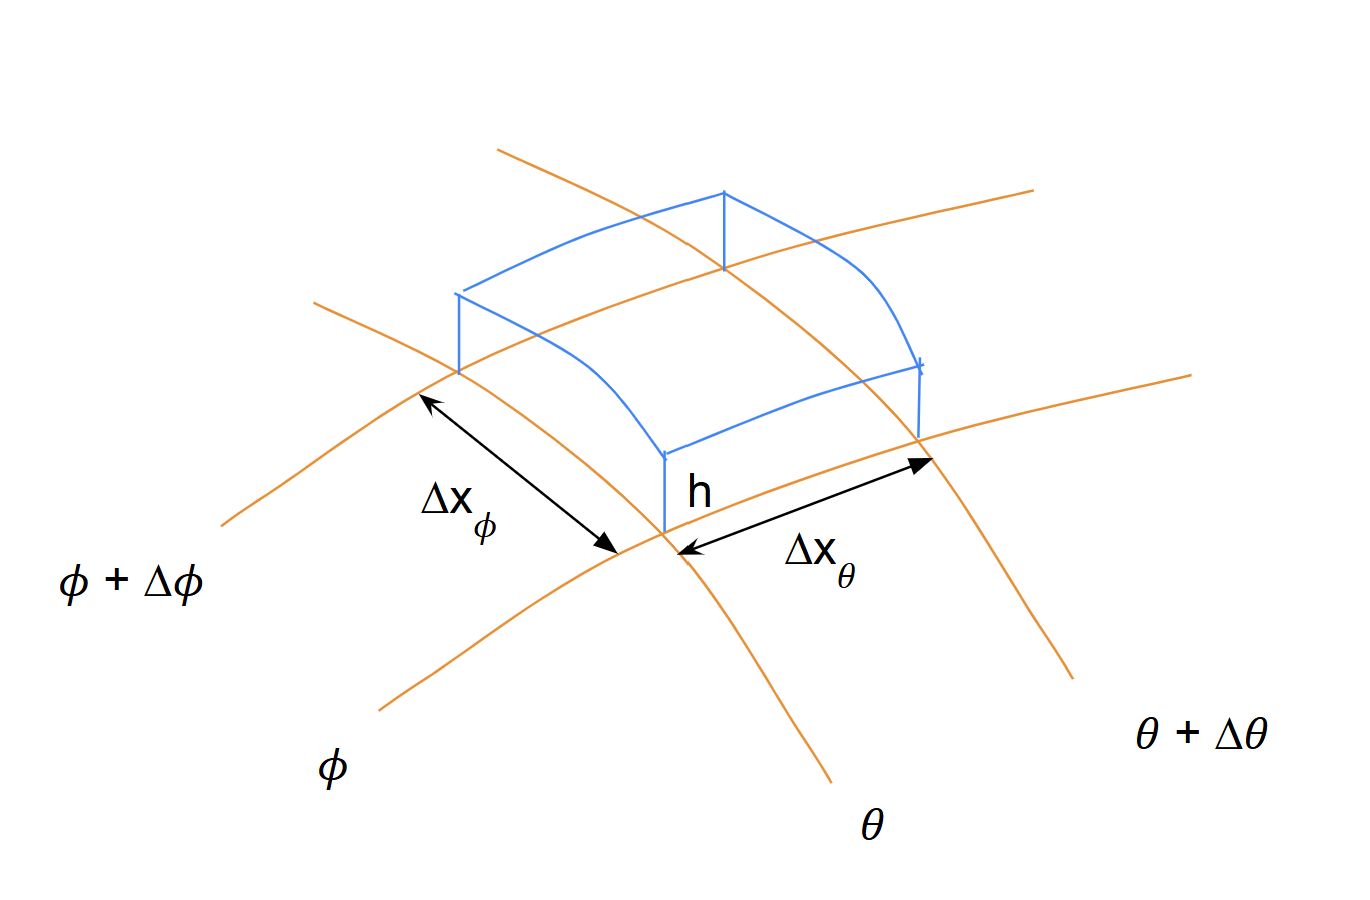
\includegraphics[width=0.5\textwidth]{C:/Users/Matteo/Shallow-Water-Equations/figs/Sphere-small-domain.png}
    \caption{Illustrations of a small domain of the surface of the sphere.}\label{fig:sphere-small-domain}
\end{figure}
The volume of the domain in~\autoref{fig:sphere-small-domain} is denoted by $V$.
To find the volume, we need to find expressions for $\Delta x_{\phi}$ and $\Delta x_{\theta}$, the distances in the $\phi$ and $\theta$ directions, respectively, as illustrated in \autoref{fig:sphere-small-domain}.
We can find these distances by using the arc length formula.
Recall that the circumreference of a full circle is $2\pi r$, where $r$ is the radius of the circle.
The arc length is a fraction of the full circumreference, and it is given by the formula $l = r v$, where $l$ is the arc length, $r$ is the radius, and $v$ is the angle in radians.
Assuming Earth's latitude side is a circle, we can find the distance $\Delta x_{\phi}$ by using the arc length formula, as:
\begin{align*}
    \Delta x_{\phi} = r \Delta \phi,
\end{align*}
where $\Delta \phi$ is the change in the latitude angle and $r$ is the radius of the sphere.
We assume that Earth is a perfect sphere, meaning that the radius is constant.
Considering the distance in the longitude dimension $\Delta x_{\theta}$, we need to make some adjustments, as we can see that the circumreference at equator is larger than at the poles.
That is, we need to consider the radius of the circle at the given latitude $\phi$.
To illustrate this, we consider \autoref{fig:sphere_r_lat}.
\begin{figure}[H]
    \centering
    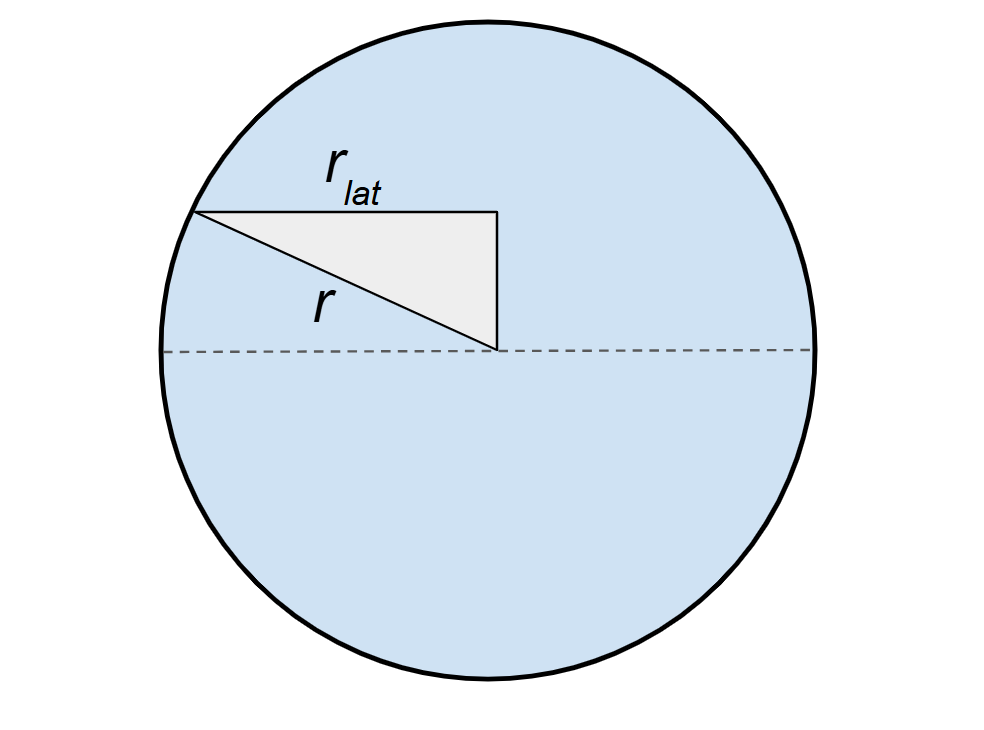
\includegraphics[width=0.4\textwidth]{C:/Users/Matteo/Shallow-Water-Equations/figs/sphere_r_lat.png}
    \caption{Illustration of the radius of the circle at the given latitude $\phi$.}\label{fig:sphere_r_lat}
\end{figure}
In \autoref{fig:sphere_r_lat}, we consider a right triangle where the length of the hypotenuse is equal to the radius of the sphere.
The length of the adjacent side $r_{lat}$ is the radius of the longitude circle at the given latitude $\phi$.
By using trigonometry, we can express the radius of the circle at the given latitude $\phi$ as
\begin{align*}
    r_{lat} = r \cos(\phi).  
\end{align*}
Using that, together with the arc length formula, we can find the distance $\Delta x_{\theta}$ as:
\begin{align*}
    \Delta x_{\theta} = r \cos(\phi) \Delta \theta.
\end{align*}
We can then compute the volume of a small domain of the sphere, as shown in \autoref{fig:sphere-small-domain}.
The volume $V$ is given by 
\begin{align*}
    V &= \Delta x_{\phi} \Delta x_{\theta} h \\
    &= r^2 h \cos(\phi) \Delta \phi \Delta \theta,
\end{align*}
assuming that the height of the domain is $h$, and that the domain is rectangular.
This is a fair assumption for small values of $\Delta x_{\phi}$ and $\Delta x_{\theta}$.
We also assume that $\phi$ is not too close to the poles, as $\cos(\phi)$ will go to zero at the poles.
We are interested in the rate of change of $V$ with respect to time, and we can find this by taking the time derivative of the volume.
That is, we consider the partial derivative with respect to time of the volume $V$:
\begin{align}\label{eq:sphere-volume-time-derivative}
    \frac{\partial V}{\partial t} &= r^2 \cos(\phi) \Delta \phi \Delta \theta \frac{\partial h}{\partial t}.
\end{align}
In~\eqref{eq:sphere-volume-time-derivative} we have utilized that $r$ is constant, and that $\cos(\phi), \Delta \phi$ and $\Delta \theta$ are independent of the time $t$.
We use $u_{\theta}$ and $u_{\phi}$ to denote the velocities in the $\theta-$ and $\phi-$directions, not to be confused with partial derivatives.
We are interested in the rate at which fluid volume enters the region from the sides.
We can find this rate by considering the flux of fluid volume through the sides of the domain.
That is, we consider how much fluid volume enters the domain from the $\theta-$direction, and how much fluid volume enters the domain from the $\phi-$direction.
We also consider how much fluid volume leaves the domain in the $\theta-$ and $\phi-$directions.
The net flux of fluid volume into the domain is the difference between the influx and the outflux.
The rate of change of the volume $V$ with respect to time is equal to the net flux of fluid volume into the domain.
That is, we have that
\begin{align}\label{eq:V_t-F_net}
    V_t = F_{net, \theta} + F_{net, \phi},
\end{align}
which combined with~\eqref{eq:sphere-volume-time-derivative} gives us the equation
\begin{align}\label{eq:sphere-volume-time-combined}
    r^2 \cos(\phi) \Delta \phi \Delta \theta \frac{\partial h}{\partial t} = F_{net, \theta} + F_{net, \phi}.
\end{align}
To find the net flux in the $\theta-$ and $\phi-$directions, we consider the influx and outflux in these directions.
We calculate the influx at the $\theta-$line and the outflux at the $(\theta + \Delta \theta)-$line, see \autoref{fig:sphere-small-domain}, to find the net flux.
The influx is the area of the $\theta$ line times the velocity in the $\theta$ direction at the $\theta$ line.
Thus, the influx in the $\theta$-direction is given by
\begin{align*}
    F_{in, \theta} = u_\theta(\theta) h(\theta)  r \Delta \phi,
\end{align*}
where $h(\theta)$ is the height of the water at the $\theta-$line, assumed to be constant along the line, and $u_\theta(\theta)$ is the velocity in the $\theta-$direction at the $\theta-$line.
This way we can compute how much the volume changes due to the influx.
For the outflux we do the same just for the $(\theta + \Delta \theta)-$line, introducing the notation $\theta ' = \theta + \Delta \theta$.
The outflux is
\begin{align*}
    F_{out, \theta}
    = u_\theta(\theta + \Delta \theta) h(\theta + \Delta \theta)  r \Delta \phi
    = u_\theta(\theta') h(\theta')  r \Delta \phi
    .
\end{align*}
The net flux in the $\theta$ direction is the difference between the influx and the outflux, and is given by
\begin{align}\label{eq:sphere-net-flux-theta}
   F_{net, \theta} = F_{in, \theta} - F_{out, \theta} 
    = \left(  u_\theta(\theta) h(\theta) - u_\theta(\theta ') h(\theta ') \right)  r \Delta \phi.
\end{align}
We can do the same for the $\phi$ direction, also using the notation $\phi ' = \phi + \Delta \phi$.
Hence, we obtain the net flux in the $\phi$ direction as
\begin{equation}\label{eq:sphere-net-flux-phi}
    \begin{aligned}
        F_{net, \phi} &= F_{in, \phi} - F_{out, \phi} \\
        &= \left( u_\phi(\phi) h(\phi)\cos (\phi) - u_\phi (\phi ')h(\phi ') \cos(\phi')  \right) r \Delta \theta.
    \end{aligned}
\end{equation}
By inserting~\eqref{eq:sphere-net-flux-theta} and~\eqref{eq:sphere-net-flux-phi} into~\eqref{eq:sphere-volume-time-combined} we can write:
\begin{align}\label{eq:sphere-volume-time-derivative-flux}
    h_t r^2 \cos(\phi) \Delta \phi \Delta \theta
    = \left( u_\theta(\theta) h(\theta) - u_\theta (\theta ')h(\theta ')  \right) r \Delta \phi
    + \left( u_\phi(\phi) h(\phi)\cos (\phi) - u_\phi (\phi ')h(\phi ') \cos(\phi')  \right) r \Delta \theta.
\end{align}
Since we are interested in $\frac{\partial h}{\partial t} = h_t$, we divide~\eqref{eq:sphere-volume-time-derivative-flux} by the area of the element, given by $r^2 \cos(\phi) \Delta \phi \Delta \theta$.
Hence we get
\begin{align}\label{eq:sphere-derivative-h}
    \frac{\partial h}{\partial t} = \frac{u_\theta(\theta) h(\theta) - u_\theta(\theta ')h(\theta ') }{r \cos(\phi) \Delta \theta} 
    + \frac{u_\phi(\phi) h(\phi)\cos (\phi) - u_\phi (\phi ')h(\phi ') \cos(\phi')}{r \cos (\phi) \Delta \phi},
\end{align}
where $\phi \neq \pm \frac{\phi}{2}$.
By collecting terms to the left hand side and changing the order of the numerators, we can rewrite~\eqref{eq:sphere-derivative-h} as 
\begin{align}\label{eq:sphere-derivative-h-collected}
    \frac{\partial h}{\partial t} + \frac{u_\theta(\theta') h(\theta') - u_\theta(\theta)h(\theta) }{r \cos(\phi) \Delta \theta} 
    + \frac{u_\phi(\phi ')h(\phi ') \cos(\phi') - u_\phi(\phi) h(\phi) \cos(\phi) }{r \cos (\phi) \Delta \phi} = 0.
\end{align}
Next step is to investigate the limit values, as $\Delta \theta$ and $\Delta \phi$ approaches zero.
We can find the limit values by using the definition of the derivative.
The derivative of a function $f(x)$ with respect to $x$ is defined as
\begin{align*}
    f'(x) = \lim_{\Delta x \to 0} \frac{f(x + \Delta x) - f(x)}{\Delta x}.
\end{align*}
We can use this definition to find the limit values in~\eqref{eq:sphere-derivative-h-collected} as
\begin{align*}
    \lim_{\Delta \theta \to 0} \frac{ u_\theta(\theta ')h(\theta ') - u_\theta(\theta) h(\theta) }{\Delta \theta} = \frac{\partial}{\partial \theta} (h u_\theta ),
\end{align*}
and 
\begin{align*}
    \lim_{\Delta \phi \to 0} \frac{ u_\phi(\phi ')h(\phi ') \cos(\phi') - u_\phi(\phi) h(\phi) \cos(\phi) }{\Delta \phi} =  \frac{\partial}{\partial \phi} (h u_\phi \cos(\phi)).
\end{align*}
Inserting these results in~\eqref{eq:sphere-derivative-h-collected} yields
\begin{align*}
    h_t + \frac{1}{r \cos (\phi)} \left( {(h u_\theta)}_{\theta} + {(h u_{\phi} \cos(\phi))}_{\phi}  \right) = 0,
\end{align*}
which is the mass conservation equation in spherical coordinates and is the first equation in the SWE in spherical coordinates.
The next step is to derive the momentum equations in spherical coordinates.
In this case, we focus on the horizontal velocity components, specifically the velocity tangential to the surface of the sphere, i.e., the $\theta$ and $\phi$ velocities.
The vertical velocity is neglected, as the key assumption in the shallow water equations is that the vertical component of the acceleration is negligible.
Additionally, when considering Earth, the water layer is thin compared to the radius of the Earth, referred to as a thin-layer approximation.
We need to express the horizontal velocity $u_h$, which is dependent on the variables $\theta, \phi$ and $t$.
Since $\theta$ and $\phi$ are angles, we introduce the unit vectors $\mathbf{e}_\theta$ and $\mathbf{e}_\phi$ on the surface in the $\theta-$ and $\phi-$directions.
The unit vectors are illustrated in~\autoref{fig:sphere-unit-vectors}.
\begin{figure}[H]
    \centering
    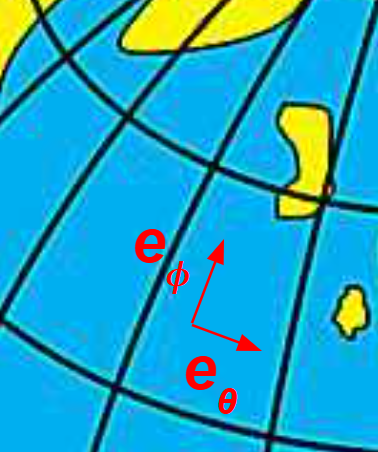
\includegraphics[width=0.2\textwidth]{C:/Users/Matteo/Shallow-Water-Equations/figs/sphere-unit-vectors.png}
    \caption{Illustration of the unit vectors $\mathbf{e}_\theta$ and $\mathbf{e}_\phi$, tangential to the surface.}\label{fig:sphere-unit-vectors}
\end{figure}
We can express the horizontal velocity $u_h$ in terms of the unit vectors as
\begin{align}\label{eq:sphere-horizontal-velocity}
    u_h(\theta, \phi, t) = u_\theta \mathbf{e}_\theta + u_\phi \mathbf{e}_\phi.
\end{align}
We are then interested in the total derivative of the horizontal velocity $u_h$ in~\eqref{eq:sphere-horizontal-velocity} with respect to time.
The total derivative is given by
\begin{align}\label{eq:sphere-total-derivative}
    \frac{\text{d}u_h}{\text{d}t} = \frac{\partial u_h}{\partial t} + \frac{\text{d}\theta}{\text{d}t} \frac{\partial u_h}{\partial \theta} + \frac{\text{d}\phi}{\text{d}t} \frac{\partial u_h}{\partial \phi}.
\end{align}
If we differentiate the longitude angle $\theta$ with respect to time, we get the angular velocity $\omega_\theta$ in the $\theta$ direction, i.e.,
\begin{align*}
    \frac{\text{d}\theta}{\text{d}t} = \omega_\theta,
\end{align*}
meaning that if $\omega_\theta > 0$, the point is moving eastwards, and if $\omega_\theta < 0$, the point is moving westwards.
Similarly, if we differentiate the latitude angle $\phi$ with respect to time, we get the angular velocity $\omega_\phi$ in the $\phi$ direction, i.e.,
\begin{align*}
    \frac{\text{d}\phi}{\text{d}t} = \omega_\phi,
\end{align*}
meaning that if $\omega_\phi > 0$, the point is moving northwards, and if $\omega_\phi < 0$, the point is moving southwards.
By using the  derivative of the arc length formula, we get that 
\begin{align}\label{eq:sphere-arc-length}
    \frac{\text{d}\theta}{\text{d}t} =  \frac{u_\theta}{r \cos(\phi)},
    \quad \frac{\text{d}\phi}{\text{d}t} = \frac{u_\phi}{r}.
\end{align}
We can now insert~\eqref{eq:sphere-arc-length} into~\eqref{eq:sphere-total-derivative} to find the total derivative of the horizontal velocity split into the $\theta-$ and $\phi-$directions:
\begin{equation}\label{eq:sphere-total-derivative-split}
    \left.
    \begin{aligned}
        \frac{\text{d}u_\theta}{\text{d}t} = \frac{\partial u_\theta}{\partial t} + \frac{u_\theta}{r \cos(\phi)} \frac{\partial u_\theta}{\partial \theta} + \frac{u_\phi}{r} \frac{\partial u_\theta}{\partial \phi}, \\
        \frac{\text{d}u_\phi}{\text{d}t} = \frac{\partial u_\phi}{\partial t} + \frac{u_\theta}{r \cos(\phi)} \frac{\partial u_\phi}{\partial \theta} + \frac{u_\phi}{r} \frac{\partial u_\phi}{\partial \phi}.
    \end{aligned}
    \right\}
\end{equation}
We know that the right hand side of~\eqref{eq:sphere-total-derivative-split} are the given physical forces acting on the fluid.
Earlier in this project, we focused on the shallow water equations in cartesian coordinates, accounting solely for gravitational forces.
However, in spherical coordinates, additional physical forces must be considered.
These could be forces like the Coriolis force, centripetal acceleration, and the effects of Earth's curvature.
First we consider the gravitational force acting on the fluid, descibed as $-g \nabla h$, where $g$ is the gravity acceleration, and $\nabla h$ is the gradient of the height $h$.
We consider the gradient of $h$:
\begin{equation*}
    \begin{aligned}
        \nabla h &= \frac{\partial h}{\partial x_\theta} \mathbf{e}_{\theta} + \frac{\partial h}{\partial x_\phi} \mathbf{e}_{\phi} \\
        &= \frac{1}{r \cos(\phi)} h_{\theta} \mathbf{e}_{\theta} + \frac{1}{r } h_{\phi} \mathbf{e}_{\phi},
    \end{aligned}
\end{equation*}
meaning that the gravity force acting on the fluid in the $\theta$ and $\phi$ directions are given by:
\begin{equation*}
    \left.
    \begin{aligned}
        &\theta-\text{direction:} \quad -\frac{g}{r \cos(\phi)} h_{\theta},\\
        &\phi-\text{direction:} \quad -\frac{g}{r} h_{\phi}.
    \end{aligned}
    \right\}
\end{equation*}
Hence, we obtain the two momentum equations in spherical coordinates as
\begin{equation}\label{eq:spherical-swe_part0} 
    \left.
    \begin{aligned}
         {(u_\theta)}_t + \frac{u_\theta}{r \cos(\phi)} {(u_\theta)}_\theta + \frac{u_\phi}{r} {(u_\theta)}_\phi = -\frac{g}{r \cos(\phi)} h_{\theta} + \text{other forces}, \\
        {( u_\phi)}_t + \frac{u_\theta}{r \cos(\phi)} {(u_\phi)}_\theta   + \frac{u_\phi}{r} {(u_\phi)}_\phi = -\frac{g}{r} h_{\phi} + \text{other forces}.
    \end{aligned}
    \right\}
\end{equation}
The next force we consider is the Coriolis force, which is a force that acts on moving objects on the surface of the earth~\cite{Coriolis}.
The Coriolis force is given by $f = 2 \Omega \sin(\phi)$, where $\Omega$ is the angular velocity of the earth.
The Coriolis force in the $\theta$ and $\phi$ directions are then given by:
\begin{equation*}
    \left.
    \begin{aligned}
        &\theta-\text{direction:} \quad f u_\phi,\\
        &\phi-\text{direction:} \quad -f u_\theta.
    \end{aligned}
    \right\}
\end{equation*}
The last thing we need to take into account when working in the spherical domain is the curvature of the earth.
This adds the following terms:
\begin{equation*}
    \left.
    \begin{aligned}
        &\theta-\text{direction:} \quad \frac{u_\theta u_\phi}{r} \tan(\phi),\\
        &\phi-\text{direction:} \quad -\frac{u_\theta^2}{r} \tan(\phi).
    \end{aligned}
    \right\}
\end{equation*}
There are several formulations of the SWE in spherical coordinates.
Inserting these forces into the momentum equations~\eqref{eq:spherical-swe_part0}, we get the following formulation of the shallow water equations in spherical coordinates:
\begin{equation}\label{eq:spherical-swe}
    \left.
    \begin{aligned}
        h_t + \frac{1}{r \cos (\phi)} \left( {(h u_\theta)}_{\theta} + {(h u_{\phi} \cos(\phi))}_{\phi}  \right) &= 0, \\
        {(u_{\theta})}_t  + \frac{u_\theta}{r \cos (\phi)} {(u_\theta)}_\theta + \frac{u_\phi}{r} {(u_\theta)}_{\phi}
        - \frac{u_\theta u_\phi }{r} \tan(\phi) + \frac{g}{r \cos (\phi)} h_\theta - f u_\phi &= 0, \\
        {(u_{\phi})}_t  + \frac{u_\theta}{r \cos (\phi)} {(u_\phi)}_\theta + \frac{u_\phi}{r} {(u_\phi)}_{\phi}
        + \frac{u_\theta^2}{r} \tan(\phi) + \frac{g}{r} h_\phi + f u_\theta &= 0,
    \end{aligned}
    \right\}
\end{equation}
where $r$ is the radius, $(\theta, \phi)$ are the longitude and latitude angles, $h$ is the height of the water, $u_\theta$ and $u_\phi$ are the velocities in the $\theta-$ and $\phi-$directions and $g$ is the gravitational constant.
We can also write the spherical SWE~\eqref{eq:spherical-swe} in vector form as
\begin{align}
    \mathbf{U}_t + \frac{1}{r \cos(\phi)} \mathbf{F(U)}_\theta + \frac{1}{r} \mathbf{G(U)}_\phi = \mathbf{S},
\end{align}
where $\frac{1}{r \cos(\phi)} \mathbf{F(U)}_\theta$ and $\frac{1}{r} \mathbf{G(U)}_\phi$ are the flux terms in the $\theta-$ and $\phi-$directions and $\mathbf{S}$ is the source term.

%Obtain in vector form:
%Multiply with $\cos \phi$ and something else. Consider the paper.

%Vector form:
%\begin{align}
%    \cos(\phi) \mathbf{U}_t + \mathbf{F(U)}_\theta + \cos(\phi) \mathbf{G(U)}_\phi = 0,
%\end{align}
%where 
%\begin{align*}
%    \mathbf{U} = \begin{bmatrix} h \\ h u_\theta \\h u_\phi \end{bmatrix},
%    \mathbf{F(U)} = \begin{bmatrix} h u_\theta \\ h u_\theta^2 + g h^2  \\ h u_\theta u_\phi \end{bmatrix},
%    \mathbf{G(U)} = \begin{bmatrix} h u_\phi \\ h u_\theta u_\phi \\ h u_\phi^2 + \ g h^2 \end{bmatrix}.
%\end{align*}


\section{The Linearized Shallow Water Equations in Spherical Coordinates}
In this section, we derive the linearized shallow water equations (LSWE) in spherical coordinates, from the nonlinear SWE in spherical coordinates, given in~\eqref{eq:spherical-swe}.
The derivation and methodology presented here are based on the sources~\cite{BONEV_2018} and~\cite{Eskilsson_2005}.
The LSWE are employed for their simplicity, providing a foundation for understanding wave dynamics in a spherical geometry.
Later in this project, we will apply the FVM to solve these equations numerically.
We focus on one spatial dimension, namely the longitude $\theta$. 
This approach assumes a constant latitude $\phi$, which simplifies the equations to a one-dimensional framework.
Hence we can neglect the third equation in~\eqref{eq:spherical-swe} and the velocity component $u_\phi$.
Thus, we introduce $u = u_\theta$ to denote the fluid velocity in the $\theta$ direction.
We also neglect all external forces, except for the gravitational force.
Thus we have the following SWE in spherical coordinates for one spatial dimension:
\begin{equation}\label{eq:spherical-swe-1D}
    \left.
    \begin{aligned}
        h_t + \frac{1}{r \cos (\phi)}  {(h u)}_{\theta}  &= 0, \\
        {u}_t  + \frac{u}{r \cos (\phi)} {u}_\theta + \frac{g}{r \cos (\phi)} h_\theta  &= 0.
    \end{aligned}
    \right\}
\end{equation}
To perfom the linearization, we use perturbation theory, meaning we assume that the water height $h$ and the velocity $u$ are small perturbations from a state of rest.
Let the perturbations in water height and velocity be represented by:
\begin{align}\label{eq:perturbations}
    h = h_0 + h', \quad u = u_0 + u',
\end{align}
where $h_0$ and $u_0$ are the equilibrium height and velocity, and $h'$ and $u'$ are the perturbations.
We assume that the equilibrium height $h_0$ is constant and that the equilibrium velocity $u_0$ is zero.
By substituting the perturbed variables~\eqref{eq:perturbations} into the 1D spherical SWE~\eqref{eq:spherical-swe-1D} and utilizing that $u_0 = 0$, we obtain
\begin{equation}\label{eq:linearized_swe_spherical-perturbations}
    \left.
    \begin{aligned}
        {(h_0 + h')}_t + \frac{1}{r \cos (\phi)} \left( (h_0 + h'){(u')}_\theta  + {(h_0 + h')}_\theta(u') \right) = 0, \\
        {(u')}_t + \frac{u'}{r \cos (\phi)} {(u')}_\theta + \frac{g}{r \cos (\phi)} h'_\theta = 0.
    \end{aligned}
    \right\}
\end{equation}
We neglect the terms involving products of pertubations arising in~\eqref{eq:linearized_swe_spherical-perturbations}, as they are second-order terms.
Hence, we obtain the LSWE in spherical coordinates with one spatial dimension $\theta$ and time $t$ as:
\begin{equation}\label{eq:linearized_swe_spherical}
    \left.
    \begin{aligned}
        h'_t + \frac{h_0}{r \cos(\phi)} u'_\theta &= 0, \\
        u'_t + \frac{g}{r \cos(\phi)} h'_\theta &= 0.
    \end{aligned}
    \right\}
\end{equation}
These equations describe the evolution of small perturbations in water height and velocity on a spherical surface.
We can also write the spherical LSWE in vector form as
\begin{align}\label{eq:linearized_swe_spherical_vector}
    \mathbf{W}_t + \mathbf{A} \mathbf{W}_\theta = 0,
\end{align}
where $\mathbf{W} =
\begin{bmatrix} h' \\ u' \end{bmatrix}$ and the coefficient matrix $\mathbf{A}$ is constant and given as:
$\mathbf{A} = \begin{bmatrix} 0 & \frac{h_0}{r \cos(\phi)} \\ \frac{g}{r \cos (\phi)} & 0 \end{bmatrix}$.


\subsubsection*{Integral form of the 1D spherical LSWE}
As in the previous sections it is beneficial to state the integral form of the 1D spherical LSWE, as it will be used when deriving the finite volume scheme.
We consider the longitude $\theta$ as the spatial dimension on a full circle, meaning the domain is $[0, 2\pi]$ radians.
The domain is divided into $N$ cells or control volumes, that each has a length of $\Delta \theta = \frac{2\pi}{N}$ radians.
We consider a control volume $V$ with cell interfaces at $\theta_L$ and $\theta_R$, as illustrated in~\autoref{fig:sphere1d_small_domain}.
\begin{figure}[H]
    \centering
    \begin{subfigure}{0.4\textwidth}
        \centering
        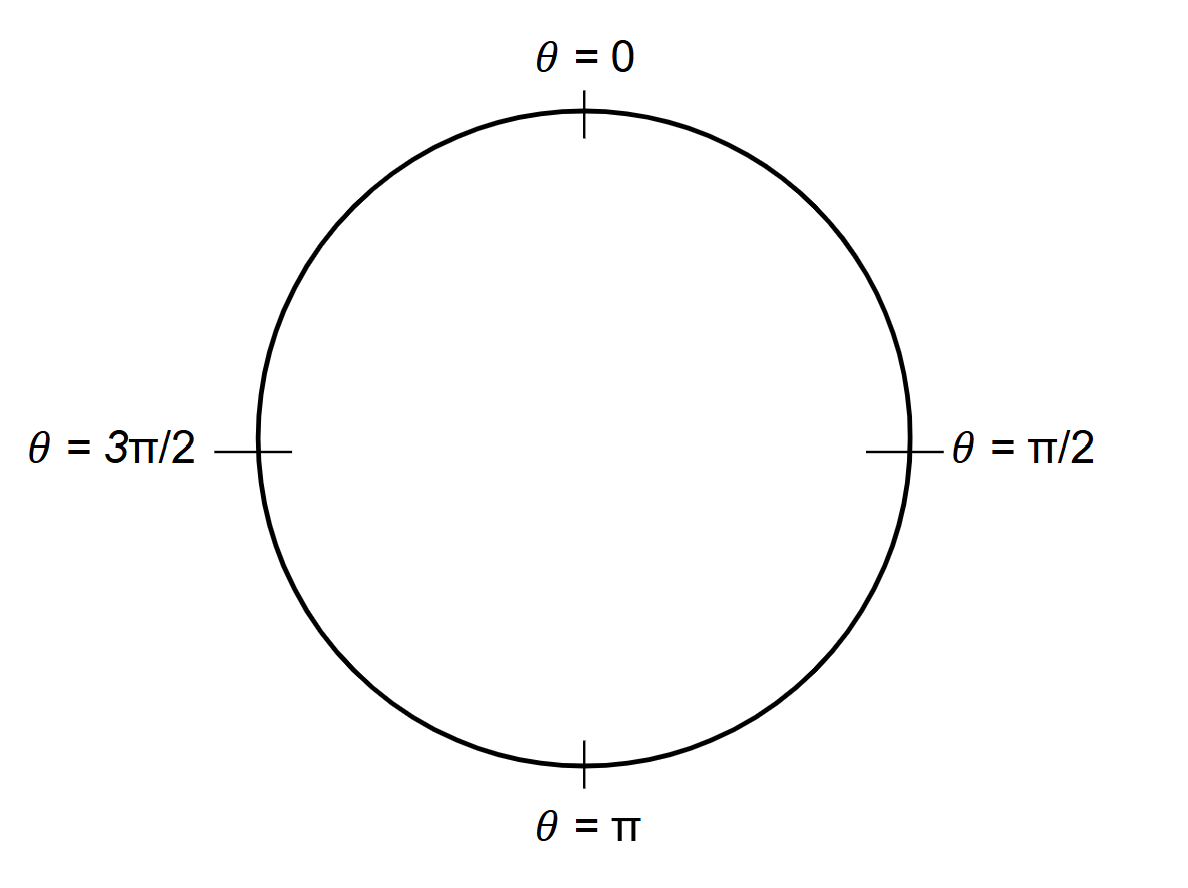
\includegraphics[width=\textwidth]{C:/Users/Matteo/Shallow-Water-Equations/figs/sphere1d_small_cell.png}
        \caption{Illustration of the grid for the 1D SWE with small cells.}\label{fig:sphere1d_small_cell}
    \end{subfigure}%
    \hspace{1cm}
    \begin{subfigure}{0.3\textwidth}
        \centering
        \raisebox{15mm}{
        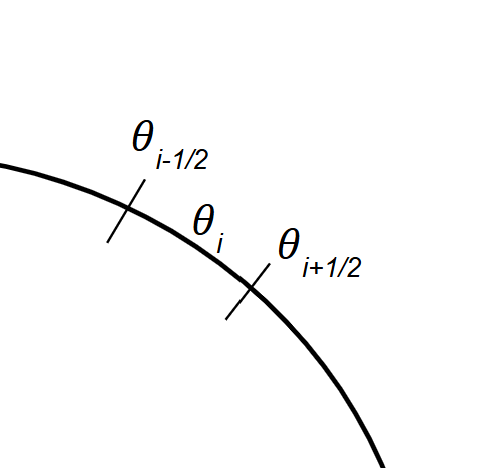
\includegraphics[width=0.9\textwidth]{C:/Users/Matteo/Shallow-Water-Equations/figs/sphere-1d-small-domain.png}
        }
        \caption{Illustration of the grid for the 1D SWE with a small domain.}\label{fig:sphere1d_small_domain}
    \end{subfigure}
    \caption{Grid illustrations for the 1D LSWE in spherical coordinates.}\label{fig:sphere1d_combined}
\end{figure}
In \autoref{fig:sphere1d_small_cell}, we see the circle, which is the full domain, and in \autoref{fig:sphere1d_small_domain} we see a small subdomain of the circle.

The integral form of the LSWE is obtained by integrating the control volume given by $V = [\theta_L, \theta_R] \times [t_1, t_2]$, where $t_2$ denotes the time step after $t_1$, over space and time. 
We begin by integrating the vector form of the 1D spherical LSWE in~\eqref{eq:linearized_swe_spherical_vector} over the spatial dimension $\theta$ from $\theta_L$ to $\theta_R$ to obtain
\begin{align}\label{eq:integral_form_spherical_1D_part0}
    \int_{\theta_L}^{\theta_R} \mathbf{W}_t \text{ d}\theta + \int_{\theta_L}^{\theta_R} \mathbf{A} \mathbf{W}_\theta \text{ d}\theta = 0.
\end{align}
Since the matrix $\mathbf{A}$ is constant, we can place it outside of the integral in~\eqref{eq:integral_form_spherical_1D_part0} to get
\begin{align}\label{eq:integral_form_spherical_1D_part1}
    \int_{\theta_L}^{\theta_R} \mathbf{W}_t \text{ d}\theta + \mathbf{A} \int_{\theta_L}^{\theta_R} \mathbf{W}_\theta \text{ d}\theta = 0.
\end{align}
We use the fundamental theorem of calculus to rewrite~\eqref{eq:integral_form_spherical_1D_part1} as
\begin{align}\label{eq:derive_integral_form_1D_spherical}
    \int_{\theta_L}^{\theta_R} \mathbf{W}_t \text{ d}\theta =  \mathbf{A} \left( \mathbf{W}(\theta_L, t) - \mathbf{W}(\theta_R, t) \right).
\end{align}
We then integrate~\eqref{eq:derive_integral_form_1D_spherical} over time from $t_1$ to $t_2$ to get
\begin{align}\label{eq:integral_form_spherical_1D_part2}
    \int_{t_1}^{t_2} \int_{\theta_L}^{\theta_R} \mathbf{W}_t \text{ d}\theta \text{ d}t = \mathbf{A} \left( \int_{t_1}^{t_2} \mathbf{W}(\theta_L, t) \text{ d}t - \int_{t_1}^{t_2} \mathbf{W}(\theta_R, t) \text{ d}t \right).
\end{align}
Rewriting~\eqref{eq:integral_form_spherical_1D_part2} gives
\begin{align}\label{eq:integral_form_spherical_1D_final}
    \int_{\theta_L}^{\theta_R} \mathbf{W}(\theta, t_2) \text{ d}\theta = \int_{\theta_L}^{\theta_R} \mathbf{W}(\theta, t_1) \text{ d}\theta
    - \mathbf{A} \left( \int_{t_1}^{t_2} \mathbf{W}(\theta_R, t) \text{ d}t - \int_{t_1}^{t_2} \mathbf{W}(\theta_L, t) \text{ d}t \right),
\end{align}
which we refer to as the integral form of the LSWE in spherical coordinates with one spatial dimension.
The integral form~\eqref{eq:integral_form_spherical_1D_final} is the foundation for the FVM, which can be used to solve the LSWE in spherical coordinates numerically.



